% ===================================================================
%  Week 9 — Session 1: Finding Contours & Basic Measurements
% ===================================================================
\documentclass[10pt,aspectratio=169]{beamer}
% ===================================================================
%  Shared Beamer preamble for "Practical Image Processing"
%  English slides. Compile with pdfLaTeX.
% ===================================================================

\usetheme{metropolis}
\usepackage[T1]{fontenc}
\usepackage[utf8]{inputenc}
\usepackage{lmodern}
\usepackage{listings}
\usepackage{tcolorbox}
\usepackage{fontawesome5}
\usepackage{booktabs}
\usepackage{amsmath,amssymb}
\usepackage{tikz}
\usepackage{pgfplots}
\pgfplotsset{compat=1.17}
\usetikzlibrary{arrows.meta,positioning,shapes.geometric,fit,backgrounds,matrix}
\tcbuselibrary{skins,breakable}

% ---- Palette --------------------------------------------------------
\definecolor{coursePrimary}{HTML}{1B4965}   % deep blue
\definecolor{courseAccent}{HTML}{E76F51}    % coral
\definecolor{courseGood}{HTML}{2A9D8F}      % teal
\definecolor{courseBad}{HTML}{C0392B}       % red
\definecolor{courseInfo}{HTML}{2980B9}      % blue
\definecolor{codeBg}{HTML}{F5F6FA}
\definecolor{codeKw}{HTML}{8E44AD}
\definecolor{codeStr}{HTML}{2A9D8F}
\definecolor{codeCom}{HTML}{7F8C8D}

\setbeamercolor{frametitle}{bg=coursePrimary}
\setbeamercolor{progress bar}{fg=courseAccent}
\setbeamercolor{alerted text}{fg=courseAccent}
\metroset{block=fill,sectionpage=progressbar,numbering=fraction}

% ---- Code listings (Python is built into listings) -----------------
\lstdefinestyle{course}{
  backgroundcolor=\color{codeBg},
  basicstyle=\ttfamily\scriptsize,
  keywordstyle=\color{codeKw}\bfseries,
  stringstyle=\color{codeStr},
  commentstyle=\color{codeCom}\itshape,
  numberstyle=\tiny\color{codeCom},
  numbers=left, numbersep=6pt,
  showstringspaces=false, breaklines=true, breakatwhitespace=true,
  tabsize=4, columns=fullflexible,
  frame=single, framesep=4pt, rulecolor=\color{gray!30},
  keepspaces=true, upquote=true, language=Python,
}
\lstset{style=course}
\lstdefinelanguage{bash}{
  keywords={cd,pip,python,venv,source,import}, sensitive=true,
  morecomment=[l]{\#}, morestring=[b]', morestring=[b]",
}

% ---- Reusable callout boxes ----------------------------------------
\newtcolorbox{goodbox}[1][Good practice]{colback=courseGood!8,colframe=courseGood,
  fonttitle=\bfseries,title={\faCheck~#1},boxrule=0.6pt,left=4pt,right=4pt,top=3pt,bottom=3pt}
\newtcolorbox{badbox}[1][Pitfall]{colback=courseBad!8,colframe=courseBad,
  fonttitle=\bfseries,title={\faTimes~#1},boxrule=0.6pt,left=4pt,right=4pt,top=3pt,bottom=3pt}
\newtcolorbox{infobox}[1][Note]{colback=courseInfo!8,colframe=courseInfo,
  fonttitle=\bfseries,title={\faInfoCircle~#1},boxrule=0.6pt,left=4pt,right=4pt,top=3pt,bottom=3pt}
\newtcolorbox{mathbox}[1][Math]{colback=coursePrimary!6,colframe=coursePrimary,
  fonttitle=\bfseries,title={\faCalculator~#1},boxrule=0.6pt,left=4pt,right=4pt,top=3pt,bottom=3pt}

\newcommand{\keyidea}[1]{\begin{alertblock}{Key idea}#1\end{alertblock}}
\newcommand{\term}[1]{\textbf{\color{coursePrimary}#1}}
\newcommand{\code}[1]{\lstinline[basicstyle=\ttfamily\small]|#1|}

% ---- A helper to draw a small pixel grid, cells shaded by value ----
% \pixelgrid{ {10,20,120,200,240}, {30,60,130,180,230}, ... }
\newcommand{\pixelgrid}[1]{%
  \begin{tikzpicture}[font=\scriptsize,scale=0.6]
    \foreach \row [count=\ry] in {#1} {
      \foreach \val [count=\cx] in \row {
        \draw[gray,fill=coursePrimary!8] (\cx,-\ry) rectangle ++(1,-1);
        \node at (\cx+0.5,-\ry-0.5) {\val};
      }
    }
  \end{tikzpicture}}


\title{Contours \& Shape Analysis}
\subtitle{Week 9 — Session 1: Finding contours \& basic measurements}
\author{Practical Image Processing}
\date{Lecture 9.1 \textbullet\ 60--70 min}

\begin{document}

\maketitle

\begin{frame}{Recap \& today}
  \begin{columns}[T]
    \begin{column}{0.58\textwidth}
      \begin{itemize}
        \item Wk8: segmentation gave us separated regions/blobs — a clean binary mask.
        \item \alert{Today (Session 1):} turn that mask into a list of \term{objects}. We
              trace \term{contours} and take the first, most useful \term{measurements}:
              area, perimeter, bounding box, centroid.
        \item Session 2 goes on to shape \emph{descriptors} and invariant matching.
      \end{itemize}
    \end{column}
    \begin{column}{0.42\textwidth}
      \begin{alertblock}{DocScan milestone}
        Find each digit's contour and crop it by its bounding box — the step that hands clean,
        ordered digits to the reader (Week 13).
      \end{alertblock}
    \end{column}
  \end{columns}
\end{frame}

\begin{frame}{Roadmap}\tableofcontents\end{frame}

% ==================================================================
\section{From regions to objects}
% ==================================================================

\begin{frame}{Where we are in the pipeline}
  \begin{center}
  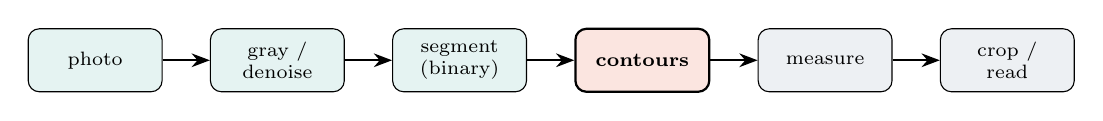
\begin{tikzpicture}[font=\scriptsize,node distance=6mm,
      box/.style={draw,rounded corners,fill=coursePrimary!8,minimum height=8mm,minimum width=17mm,align=center},
      done/.style={draw,rounded corners,fill=courseGood!12,minimum height=8mm,minimum width=17mm,align=center},
      now/.style={draw,rounded corners,fill=courseAccent!18,thick,minimum height=8mm,minimum width=17mm,align=center},
      a/.style={-{Stealth[]},thick}]
    \node[done] (raw) {photo};
    \node[done,right=of raw] (gray) {gray /\\denoise};
    \node[done,right=of gray] (bin) {segment\\(binary)};
    \node[now,right=of bin] (cnt) {\textbf{contours}};
    \node[box,right=of cnt] (meas) {measure};
    \node[box,right=of meas] (read) {crop /\\read};
    \draw[a] (raw)--(gray); \draw[a] (gray)--(bin); \draw[a] (bin)--(cnt);
    \draw[a] (cnt)--(meas); \draw[a] (meas)--(read);
  \end{tikzpicture}
  \end{center}
  \begin{itemize}
    \item A binary mask is still just \emph{pixels}. We want a list of \term{things}: ``9 digits, here are their positions and sizes.''
    \item Contours are the bridge from a pixel grid to countable, measurable objects.
  \end{itemize}
\end{frame}

\begin{frame}{A contour = the outline of a region}
  \begin{columns}[T]
    \begin{column}{0.5\textwidth}\begin{center}
      
\includegraphics[width=0.95\linewidth]{../assets/binary.png}\\{\scriptsize binary digits}\\[4pt]
      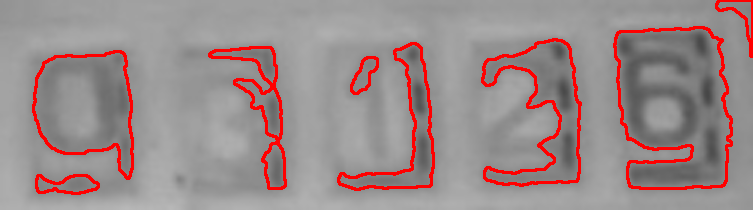
\includegraphics[width=0.95\linewidth]{../assets/contours.png}\\{\scriptsize contours (red)}
    \end{center}\end{column}
    \begin{column}{0.5\textwidth}
      \begin{itemize}
        \item A \term{contour} is an ordered list of the boundary points of one connected white region.
        \item From a clean binary image, \code{findContours} walks around each object and records its outline.
        \item Each contour is one object you can measure, filter, and crop.
      \end{itemize}
      \keyidea{One binary mask $\rightarrow$ a Python list of contours, one entry per object.}
    \end{column}
  \end{columns}
\end{frame}

\begin{frame}{How border-following works (intuition)}
  \begin{columns}[T]
    \begin{column}{0.52\textwidth}
    \begin{center}
    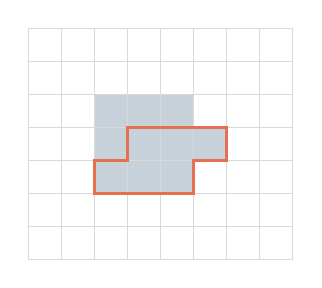
\begin{tikzpicture}[scale=0.42,font=\tiny]
      % filled region (white object pixels)
      \foreach \x/\y in {2/2,3/2,4/2,2/3,3/3,4/3,5/3,2/4,3/4,4/4}
        \fill[coursePrimary!25] (\x,\y) rectangle ++(1,1);
      % pixel grid on top
      \foreach \x in {0,...,7}\foreach \y in {0,...,6}
        \draw[gray!30] (\x,\y) rectangle ++(1,1);
      % trace arrow around the boundary
      \draw[courseAccent,very thick,-{Stealth[]}]
        (2,2)--(5,2)--(5,3)--(6,3)--(6,4)--(3,4)--(3,3)--(2,3)--cycle;
    \end{tikzpicture}
    \end{center}
    \end{column}
    \begin{column}{0.48\textwidth}
      \begin{enumerate}\scriptsize
        \item Scan the mask until you hit the first white pixel with a black neighbour — a boundary pixel.
        \item ``Walk'' around the region, always keeping the object on one side (Moore / Suzuki tracing).
        \item Record each boundary pixel in order until you return to the start.
      \end{enumerate}
      \begin{infobox}[Ordered, not a set]
        The output is a \emph{sequence} of points, so ``next point along the boundary'' is meaningful.
      \end{infobox}
    \end{column}
  \end{columns}
\end{frame}

\begin{frame}[fragile]{findContours: modes \& approximation}
\begin{lstlisting}[language=Python]
contours, hierarchy = cv2.findContours(binary,
    cv2.RETR_EXTERNAL,        # only outer contours (ignore holes)
    cv2.CHAIN_APPROX_SIMPLE)  # compress straight runs to their endpoints
\end{lstlisting}
  \begin{itemize}
    \item \term{RETR\_EXTERNAL}: outer boundaries only. \term{RETR\_TREE}: full nesting hierarchy (Session 2).
    \item \term{CHAIN\_APPROX\_NONE}: every boundary pixel. \term{CHAIN\_APPROX\_SIMPLE}: only corner points — a
          rectangle becomes 4 points, not hundreds.
    \item Input must be a \emph{binary} image; \code{contours} is a list of $N\times1\times2$ point arrays.
  \end{itemize}
\end{frame}

\begin{frame}{Retrieval modes at a glance}
  \begin{columns}[T]
    \begin{column}{0.5\textwidth}
    \begin{center}
    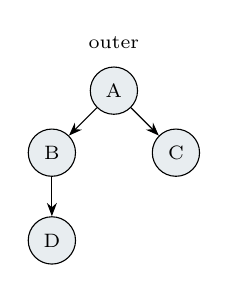
\begin{tikzpicture}[font=\scriptsize,node distance=5mm,
        n/.style={draw,circle,fill=coursePrimary!10,minimum size=6mm},
        a/.style={-{Stealth[]}}]
      \node[n](o1){A}; \node[n,below left=of o1](c1){B};
      \node[n,below right=of o1](c2){C}; \node[n,below=of c1](g1){D};
      \draw[a](o1)--(c1); \draw[a](o1)--(c2); \draw[a](c1)--(g1);
      \node[above=1mm of o1]{\scriptsize outer};
    \end{tikzpicture}\\[2pt]{\scriptsize RETR\_TREE: full parent/child tree}
    \end{center}
    \end{column}
    \begin{column}{0.5\textwidth}
      \begin{itemize}
        \item \term{RETR\_EXTERNAL}: keep A only (drop nested B, C, D).
        \item \term{RETR\_LIST}: all contours, \emph{no} hierarchy.
        \item \term{RETR\_CCOMP}: two levels (outer + holes).
        \item \term{RETR\_TREE}: the complete nesting relationship.
      \end{itemize}
      \begin{goodbox}
        For cropping isolated digits, \term{RETR\_EXTERNAL} is the simplest correct choice.
      \end{goodbox}
    \end{column}
  \end{columns}
\end{frame}

\begin{frame}{Contours vs connected components}
  \begin{itemize}
    \item \term{Connected components} label each pixel with its region id — a labelled image the size of the input.
    \item \term{Contours} give the ordered \emph{boundary} of each region — a compact list of points.
    \item Use components to count/label fast; use contours to measure shape and crop. They pair naturally.
  \end{itemize}
  \begin{center}\scriptsize
  \begin{tabular}{@{}lll@{}}
    \toprule
    & \textbf{Connected components} & \textbf{Contours} \\
    \midrule
    Output & labelled image (same size) & list of point sequences \\
    Best for & counting, per-pixel stats & shape, boxes, cropping \\
    OpenCV & \code{connectedComponents} & \code{findContours} \\
    \bottomrule
  \end{tabular}
  \end{center}
  \keyidea{Both turn a binary mask into a list of objects — the bridge from pixels to measurable things.}
\end{frame}

% ==================================================================
\section{Basic measurements}
% ==================================================================

\begin{frame}{The core measurements}
  \begin{center}
  \begin{tabular}{@{}ll@{}}
    \toprule
    \textbf{Measurement} & \textbf{OpenCV} \\
    \midrule
    Area & \code{cv2.contourArea(c)} \\
    Perimeter & \code{cv2.arcLength(c, True)} \\
    Bounding box (axis-aligned) & \code{cv2.boundingRect(c)} \\
    Rotated box & \code{cv2.minAreaRect(c)} \\
    Enclosing circle & \code{cv2.minEnclosingCircle(c)} \\
    Centroid & from \code{cv2.moments(c)} \\
    \bottomrule
  \end{tabular}
  \end{center}
  These turn a shape into numbers you can \emph{filter, sort, and compare} — the whole game this week.
\end{frame}

\begin{frame}{Area — and the shoelace formula}
  \begin{columns}[T]
    \begin{column}{0.54\textwidth}
      \begin{mathbox}[Polygon area]
        For a closed polygon with vertices $(x_i,y_i)$:
        \[ A=\tfrac12\left|\sum_{i=1}^{n}\big(x_i y_{i+1}-x_{i+1}y_i\big)\right| \]
        (indices wrap: $x_{n+1}=x_1$). This is what \code{contourArea} computes from the boundary points.
      \end{mathbox}
    \end{column}
    \begin{column}{0.46\textwidth}
      \begin{itemize}\scriptsize
        \item No need to count interior pixels — the boundary alone fixes the area.
        \item Green's theorem in disguise: a line integral around the loop gives the enclosed area.
        \item \code{contourArea} returns signed-then-absolute area; watch out for \emph{very} thin contours ($A\approx0$).
      \end{itemize}
    \end{column}
  \end{columns}
\end{frame}

\begin{frame}{Worked example: area by shoelace}
  \begin{columns}[T]
    \begin{column}{0.42\textwidth}
    \begin{center}
    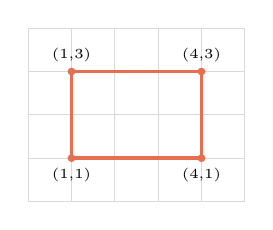
\begin{tikzpicture}[scale=0.55,font=\scriptsize]
      \draw[step=1,gray!30] (0,0) grid (5,4);
      \draw[courseAccent,very thick] (1,1)--(4,1)--(4,3)--(1,3)--cycle;
      \node[fill=courseAccent,circle,inner sep=1pt] at (1,1){};
      \node[fill=courseAccent,circle,inner sep=1pt] at (4,1){};
      \node[fill=courseAccent,circle,inner sep=1pt] at (4,3){};
      \node[fill=courseAccent,circle,inner sep=1pt] at (1,3){};
      \node[below] at (1,1){\tiny(1,1)};\node[below] at (4,1){\tiny(4,1)};
      \node[above] at (4,3){\tiny(4,3)};\node[above] at (1,3){\tiny(1,3)};
    \end{tikzpicture}
    \end{center}
    \end{column}
    \begin{column}{0.58\textwidth}
      \begin{itemize}\scriptsize
        \item Vertices in order: $(1,1),(4,1),(4,3),(1,3)$.
        \item $\sum x_i y_{i+1}=1\!\cdot\!1+4\!\cdot\!3+4\!\cdot\!3+1\!\cdot\!1=26$.
        \item $\sum x_{i+1} y_i=4\!\cdot\!1+4\!\cdot\!1+1\!\cdot\!3+1\!\cdot\!3=14$.
        \item $A=\tfrac12|26-14|=\mathbf{6}$ — matches $3\times2$. \checkmark
      \end{itemize}
      \begin{infobox}[Sanity check]
        Always cross-check a formula on a shape whose answer you already know.
      \end{infobox}
    \end{column}
  \end{columns}
\end{frame}

\begin{frame}{Perimeter (arc length)}
  \begin{itemize}
    \item \code{cv2.arcLength(c, closed=True)} sums the distances between consecutive contour points.
    \item For the box above: $3+2+3+2=\mathbf{10}$ — the loop closes back to the start.
    \item \term{CHAIN\_APPROX\_SIMPLE} keeps perimeter accurate for straight edges; curves need more points.
  \end{itemize}
  \begin{mathbox}[Perimeter]
    \( P=\sum_{i=1}^{n}\sqrt{(x_{i+1}-x_i)^2+(y_{i+1}-y_i)^2} \)
  \end{mathbox}
  \begin{badbox}
    Pass \code{closed=False} by mistake and you drop the last edge — perimeter comes out too small.
  \end{badbox}
\end{frame}

\begin{frame}{Bounding box (axis-aligned)}
  \begin{columns}[T]
    \begin{column}{0.45\textwidth}
    \begin{center}
    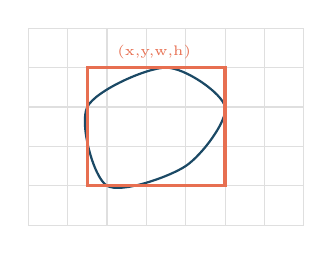
\begin{tikzpicture}[scale=0.5,font=\scriptsize]
      \draw[step=1,gray!25] (0,0) grid (7,5);
      \draw[coursePrimary,thick] plot[smooth cycle] coordinates{(2,1)(4,1.5)(5,3)(3.5,4)(1.5,3)};
      \draw[courseAccent,very thick] (1.5,1) rectangle (5,4);
      \node[courseAccent] at (3.2,4.4){\tiny (x,y,w,h)};
    \end{tikzpicture}
    \end{center}
    \end{column}
    \begin{column}{0.55\textwidth}
      \begin{itemize}\scriptsize
        \item \code{x,y,w,h = cv2.boundingRect(c)} — smallest upright rectangle containing the contour.
        \item $x,y$ = top-left corner; $w,h$ = width, height. \term{Area} of box $=w\cdot h$.
        \item The crop \code{img[y:y+h, x:x+w]} is exactly one object, ready to hand off.
        \item Cheap, robust, and the workhorse of digit cropping.
      \end{itemize}
    \end{column}
  \end{columns}
\end{frame}

\begin{frame}{Rotated box \& enclosing circle}
  \begin{columns}[T]
    \begin{column}{0.45\textwidth}
    \begin{center}
    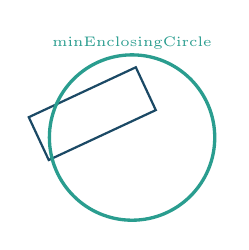
\begin{tikzpicture}[scale=0.5,font=\scriptsize]
      \draw[coursePrimary,thick,rotate=25] (1,1) rectangle (4,2.2);
      \draw[courseGood,very thick] (2.6,1.9) circle (2.1);
      \node[courseGood] at (2.6,4.3){\tiny minEnclosingCircle};
    \end{tikzpicture}
    \end{center}
    \end{column}
    \begin{column}{0.55\textwidth}
      \begin{itemize}\scriptsize
        \item \code{cv2.minAreaRect(c)} $\rightarrow$ (center, (w,h), angle): the smallest \emph{rotated} rectangle.
        \item Use it when objects are tilted (a slanted meter, a rotated document).
        \item \code{cv2.minEnclosingCircle(c)} $\rightarrow$ (center, radius): handy for round parts / coins.
      \end{itemize}
      \begin{goodbox}
        Rotated box width/height are orientation-independent — better for tilted digits than the upright box.
      \end{goodbox}
    \end{column}
  \end{columns}
\end{frame}

\begin{frame}[fragile]{Centroid from moments}
  \begin{columns}[T]
    \begin{column}{0.55\textwidth}
      \begin{mathbox}[Centroid]
        From the image moments $M_{pq}=\sum_{x,y} x^p y^q\,I(x,y)$:
        \[ \bar{x}=\frac{M_{10}}{M_{00}},\qquad \bar{y}=\frac{M_{01}}{M_{00}} \]
        $M_{00}$ is the area (mass), $M_{10},M_{01}$ the first moments.
      \end{mathbox}
    \end{column}
    \begin{column}{0.45\textwidth}
\begin{lstlisting}[language=Python,basicstyle=\ttfamily\tiny]
M = cv2.moments(c)
cx = M["m10"] / M["m00"]
cy = M["m01"] / M["m00"]
\end{lstlisting}
      \begin{itemize}\scriptsize
        \item The centroid is the shape's ``balance point.''
        \item Robust anchor for tracking, ordering, and alignment.
      \end{itemize}
    \end{column}
  \end{columns}
\end{frame}

\begin{frame}{Worked example: measure one digit}
  \begin{columns}[T]
    \begin{column}{0.4\textwidth}
      \pixelgrid{{0,0,0,0},{0,1,1,0},{0,1,1,0},{0,1,1,0},{0,0,0,0}}
    \end{column}
    \begin{column}{0.6\textwidth}
      \begin{itemize}\scriptsize
        \item White region: a $2\times3$ block of ``1'' pixels (columns 2--3, rows 2--4).
        \item \term{Area} $\approx 6$ px (pixel count) — \code{contourArea} on the boundary gives $\approx$ the same.
        \item \term{Bounding box} $w=2,\,h=3\Rightarrow$ box area $=6$, \term{extent} $=6/6=1.0$ (a solid rectangle).
        \item \term{Aspect ratio} $w/h=2/3\approx0.67$ — taller than wide, digit-like.
        \item \term{Centroid} at the block's middle: $(\bar{x},\bar{y})=(2.5,3.0)$.
      \end{itemize}
    \end{column}
  \end{columns}
  \keyidea{Six numbers now describe this blob — enough to decide ``digit or noise?''}
\end{frame}

% ==================================================================
\section{Boxes → crop, order, and filter}
% ==================================================================

\begin{frame}{Bounding boxes $\rightarrow$ crop \& order the digits}
  \begin{center}
  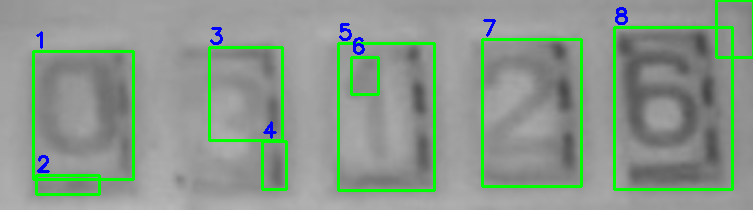
\includegraphics[width=0.8\linewidth]{../assets/boxes.png}
  \end{center}
  \begin{itemize}
    \item Draw a box around each digit; \term{sort} the boxes by their $x$-coordinate (left to right).
    \item Crop each box $\rightarrow$ one clean image per digit, \emph{in reading order}.
    \item This is exactly the DocScan hand-off to the recognizer (Week 13).
  \end{itemize}
\end{frame}

\begin{frame}[fragile]{Cropping \& ordering in code}
\begin{lstlisting}[language=Python]
boxes = [cv2.boundingRect(c) for c in contours]
boxes = sorted(boxes, key=lambda b: b[0])   # sort by x (left to right)
digits = [gray[y:y+h, x:x+w] for (x, y, w, h) in boxes]
\end{lstlisting}
  \begin{itemize}
    \item Sorting by $x$ gives the number in reading order — no OCR needed yet.
    \item For multi-row layouts, sort by $(\text{row band}, x)$: group by $y$ first, then $x$ within a row.
  \end{itemize}
  \begin{infobox}[Tie-break]
    If two boxes share an $x$, add $y$ as a secondary key: \code{key=lambda b:(b[0],b[1])}.
  \end{infobox}
\end{frame}

\begin{frame}{Filtering by shape}
  \begin{itemize}
    \item Real images give junk contours — noise specks, partial marks, a long scratch.
    \item Filter using the numbers we just computed: \term{area} (too small = noise),
          \term{aspect ratio} (digits are tallish), \term{extent} (fill fraction of the box).
    \item A handful of thresholds removes most false positives before any recognition.
  \end{itemize}
  \begin{goodbox}
    ``Keep contours with area $>$ T and $0.2 < w/h < 1.0$'' separates digits from noise robustly.
  \end{goodbox}
\end{frame}

\begin{frame}{Worked example: which blobs survive the filter?}
  \begin{center}\scriptsize
  \begin{tabular}{@{}lccccl@{}}
    \toprule
    Blob & area & w & h & w/h & keep? (area$>$200, $0.2<$w/h$<1.2$)\\
    \midrule
    digit ``7''   & 640 & 22 & 40 & 0.55 & \textcolor{courseGood}{keep} \\
    noise speck   & 18  & 5  & 4  & 1.25 & \textcolor{courseBad}{drop (area)} \\
    scratch       & 300 & 90 & 4  & 22.5 & \textcolor{courseBad}{drop (w/h)} \\
    digit ``1''   & 210 & 8  & 38 & 0.21 & \textcolor{courseGood}{keep} \\
    \bottomrule
  \end{tabular}
  \end{center}
  \begin{itemize}
    \item The speck fails on \term{area}; the scratch fails on \term{aspect ratio} — two rules, most junk gone.
    \item Thin ``1'' is a near-miss on $w/h$ — this is why thresholds need a little slack.
  \end{itemize}
\end{frame}

\begin{frame}{Pitfalls when measuring}
  \begin{badbox}
    A merged pair of digits looks like \emph{one} big contour; a broken digit looks like \emph{two}.
    Fix the mask upstream (Weeks 7--8) before trusting counts.
  \end{badbox}
  \begin{itemize}
    \item \code{contourArea} of a self-intersecting or open contour is meaningless — keep contours closed.
    \item Bounding box in \code{(x,y,w,h)}; NumPy slicing is \code{[y:y+h, x:x+w]} — row first. Easy to swap.
    \item Tiny contours can have zero area $\Rightarrow$ division by $M_{00}=0$ in the centroid. Filter first.
  \end{itemize}
\end{frame}

% ==================================================================
\section{In-class exercise}
% ==================================================================

\begin{frame}{\faPen~In-class exercise (12 min)}
  \begin{infobox}[Design the filter]
    You have contours from a meter photo: 9 digits plus some noise specks and one long scratch.
  \end{infobox}
  \begin{enumerate}
    \item Which measurements distinguish a digit from a speck? From a scratch?
    \item Write a filter rule (area + aspect ratio) that keeps digits and drops the rest.
    \item After filtering, how do you output the digits in the correct left-to-right order?
    \item What single upstream problem would break your count no matter how good the filter is?
  \end{enumerate}
\end{frame}

\begin{frame}{\faPen~Debrief}
  \begin{itemize}
    \item Speck: tiny \term{area} $\rightarrow$ drop by \code{area > T}. Scratch: extreme \term{aspect ratio} (very wide/thin) $\rightarrow$ drop.
    \item Rule: keep if \code{area>200 and 0.2<w/h<1.2} — digits are compact and tallish.
    \item Order: sort the kept bounding boxes by $x$; read left to right.
    \item Upstream killer: merged/broken digits from a bad mask — no filter recovers a missing split.
  \end{itemize}
  \keyidea{Shape measurements turn ``which blobs are digits?'' into a few numeric thresholds.}
\end{frame}

% ==================================================================
\section{Wrap-up}
% ==================================================================

\begin{frame}{What you can do after Session 1}
  \begin{itemize}
    \item Find contours; pick a retrieval mode and an approximation method.
    \item Explain the difference between contours and connected components.
    \item Measure area (shoelace), perimeter, bounding box, rotated box, and centroid.
    \item Filter contours by area / aspect ratio / extent, then crop and order digits.
  \end{itemize}
  \begin{goodbox}
    Every measurement here is one line of OpenCV — but knowing \emph{which} number to threshold is the skill.
  \end{goodbox}
\end{frame}

\begin{frame}{Next session}
  \begin{columns}[T]
    \begin{column}{0.6\textwidth}
      \begin{itemize}
        \item We can measure a shape — but our numbers change if the object rotates or scales.
        \item \alert{Session 2:} \term{shape descriptors} that are (nearly) invariant — circularity,
              solidity, moments, and \term{Hu moments} — plus convex hulls, polygon approximation,
              and contour hierarchy (holes).
        \item That's what lets DocScan find a page's 4 corners and match shapes without training.
      \end{itemize}
    \end{column}
    \begin{column}{0.4\textwidth}
      \begin{infobox}[Bring]
        Your filtered digit crops from today — Session 2 turns them into descriptors.
      \end{infobox}
    \end{column}
  \end{columns}
\end{frame}

\begin{frame}[standout]
  Contours turn regions into a list of objects.\\[4pt]
  \normalsize Find, then measure: area, perimeter, box, centroid — the numbers everything else builds on.
\end{frame}

\end{document}
